\chapter{Set Cover}
In the next recess Greg and his friends were discussing again what
to play. It was always hard to find games that everybody liked.
For example, Greg likes to play tables tennis or hide and seek but
does not want to play soccer. Suddenly Greg had an idea: What about
making a list of everybody's first and second choice and then 
finding groups which could play together. His friends agree and
you can see the result in \cref{tab:game_voting}.

\begin{table}[ht]
  \centering
  \begin{tabular}{l|cccc}
    & table tennis & hide and seek & soccer & swings \\
    \hline
    Greg  & 1 &   &   & 2 \\
    Joey  & 2 & 1 &   &   \\
    Susan & 1 &   & 2 &   \\
    Bella &   &   & 2 & 1 \\
    Jenny & 1 & 2 &   &   \\
    Jason &   &   & 1 & 2 \\
    Alice &   & 2 &   & 1 \\
    Bob   &   & 1 & 2 &   \\
  \end{tabular}
  \caption{\label{tab:game_voting}Voting of Greg and his friends}
\end{table}

Then Greg goes to Mrs. Lloyd and asks her how they could find the 
best solution. Firstly, she makes another list
(\cref{tab:example_set_cover}) where she puts all the children's
names and sums up their preferences.
\footnote{Note that I cheated here: Usually you would divide the
sum of preferences by the number of children who want to play the
game. But Greg does not know yet how to divide, so I made all the
groups have equal size.}

\begin{table}[ht]
  \centering
  \begin{tabular}{lc}
    table tennis (Greg, Joey, Susan, Jenny): & 4 \\
    hide and seek (Joey, Jenny, Alice, Bob): & 6 \\
    soccer (Susan, Bella, Jason, Bob):       & 7 \\
    swings (Greg, Bella, Jason, Alice):      & 6 \\
  \end{tabular}
  \caption{\label{tab:example_set_cover}Summed up preferences for each game}
\end{table}

\begin{figure}[ht]
  \centering
  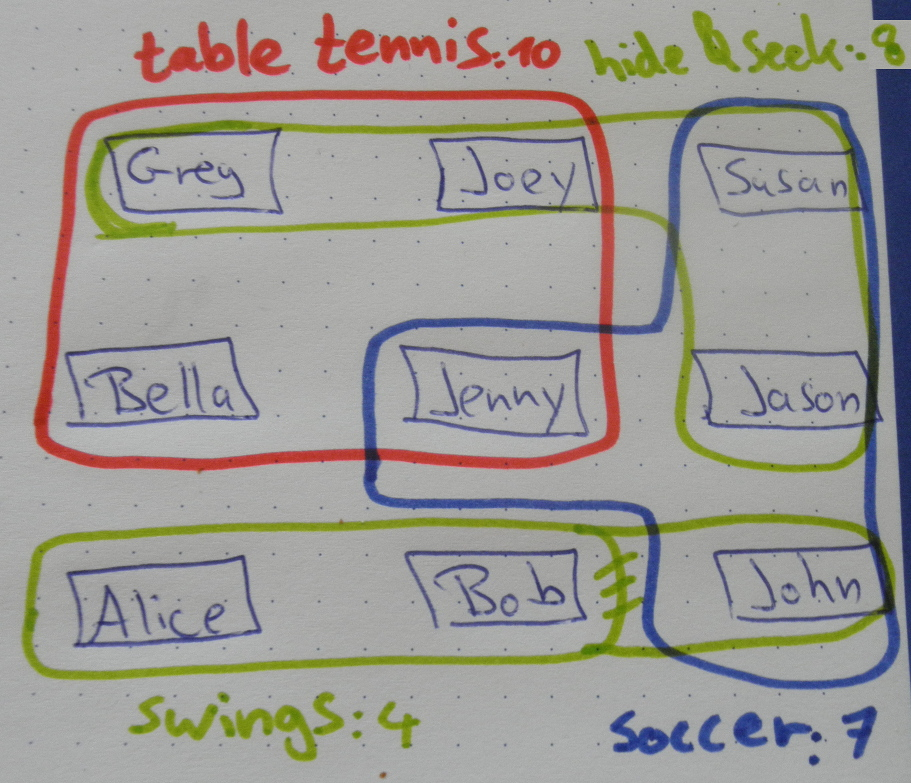
\includegraphics[width=0.5\textwidth]{img/example_set_cover.jpg}
  \caption{\label{fig:example_set_cover}Example for a set cover instance.}
\end{figure}

%--------------------------------------------------------------------##########
